 \chapter{Experimental Tasks}

\begin{figure}[ht]
\centering
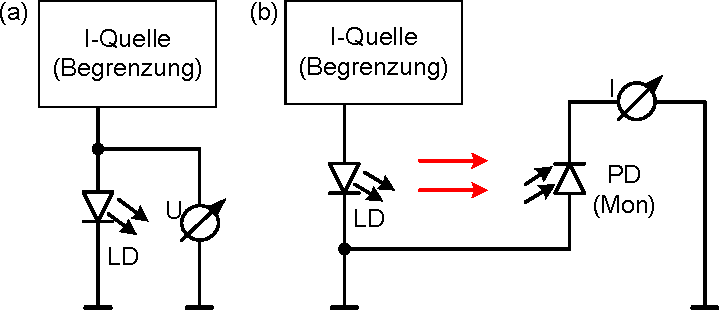
\includegraphics[width=.6\columnwidth]{Grafiken/measurement1.pdf}%
\caption{}%
\label{fig:measurement1}%
\end{figure}


\section{Recording of the U/I-Curve}



 In the first experimental task the U/I-curve of the laser diode is recorded. This is done by biasing the diode with a current and measuring the voltage (cf. Figure \ref{fig:measurement1}a). The bias current is increased from a minimum of 6.4~mA to 65~mA in steps of 2~mA. The resulting U/I-curve is shown in Figure \ref{fig:UI-curve}.

From
\begin{equation}
 \begin{split}
I = I\i{S0}\left[\e^{\beta\left(U-R\i{s}I\right)}-1\right] \hspace{2cm} I\leq I\i{S}\\
U = W\i{G}/e +R\i{S}I \hspace{2cm} I\geq I\i{S}\\
 \end{split}
\end{equation}
follows for the current above threshold:
\begin{equation}
 I = \frac{W\i{G}/e}{R\i{S}}-\frac{U}{R\i{S}} = a + b\cdot U
\end{equation}
The coefficients a and b can be determined by fitting a linear function to the U/I-curve above the threshold. The threshold current is calculated later in section \ref{ch:threshold}.  With these coefficients the band gap and the serial resistance of the laser diode can be calculated as:
\begin{equation}
\begin{split}
 W\i{G}/e=\\
 R\i{S} = 
\end{split}
\end{equation}


\section{P/I-Curve}
The output power of the laser diode at different driving currents is measured with a reference detector at the rear mirror of the laser resonator. Because the reflectivity is the same at both mirrors of the laser diode, the measured power is identical with the power emmitted in the other direction. The setup for measuring is shown in figure \ref{fig:measurement1}b.

